\documentclass[a4paper,fleqn]{cas-dc}
\usepackage[numbers,sort&compress]{natbib}
\usepackage{array}
\usepackage{CharisSIL}
\usepackage{adjustbox}
\usepackage{enumitem}
\usepackage{orcidlink}
\usepackage{placeins}
\usepackage{silence}
\WarningFilter{hyperref}{Ignoring empty anchor}


\emergencystretch=3em
\hbadness=10000

\newcommand{\apbin}[1]{\mathrm{AP}_{#1}}
\newcommand{\dAP}{\Delta\mathrm{AP}}
\newcommand{\DIFF}{\mathrm{DIFF}}
\newcommand{\SUR}{\mathrm{SUR}}
\newcommand{\best}[1]{\textbf{#1}}
\newcommand{\sigstar}{\textsuperscript{*}}
\newcommand{\AP}{\mathrm{AP}}
\newcommand{\Jclean}{\mathrm{J95}}
% Generated from corrected, primary-bound TIDE records.
\newcommand{\TideCls}{+0.382}
\newcommand{\TideLoc}{-0.004}
\newcommand{\TideBoth}{-0.019}
\newcommand{\TideDupe}{+0.018}
\newcommand{\TideBkg}{-0.154}
\newcommand{\TideMiss}{-0.321}
\newcommand{\TideCocoEval}{+0.318}
\newcommand{\TideOwnAP}{+0.187}
\newcommand{\TideCocoCls}{-0.094}
\newcommand{\TideVocCls}{+0.004}
\newcommand{\TideKittiCls}{+0.142}
\newcommand{\TideTTCls}{+1.476}

\newcolumntype{Y}[1]{>{\raggedright\arraybackslash}p{#1}}
\graphicspath{{figures/}}
\pdfstringdefDisableCommands{%
  \def\corref#1{}%
  \def\orcidlink#1{}%
}

\newcommand{\FirstPageCorrespondence}{%
  \footnotesize
  \raggedright
  \rule{2em}{0.4pt}\par
  \noindent \sigstar\ Corresponding author.\par
  \noindent \textit{E-mail addresses:}
  \href{mailto:nguyendinhthuan.st@tdtu.edu.vn}{nguyendinhthuan.st@tdtu.edu.vn}
  (D.T. Nguyen),
  \href{mailto:nguyenphuonglam.st@tdtu.edu.vn}{nguyenphuonglam.st@tdtu.edu.vn}
  (L.P. Nguyen),
  \href{mailto:nguyenvinhhuy@dtu.edu.vn}{nguyenvinhhuy@dtu.edu.vn}
  (V.H. Nguyen),
  \href{mailto:vuquangsy@tdtu.edu.vn}{vuquangsy@tdtu.edu.vn}
  (S.V. Quang),
  \href{mailto:rajeshelara@sutd.edu.sg}{rajeshelara@sutd.edu.sg}
  (M.R. Elara), and
  \href{mailto:leanhvu@tdtu.edu.vn}{leanhvu@tdtu.edu.vn}
  (A.V. Le).
}

% Keep the correspondence footer and page numeral inside the CAS media box.
\ExplSyntaxOn
\cs_set_protected:Npn \__first_foot:
  {
    \parbox[b]{\textwidth}
      {
        \FirstPageCorrespondence
        \par\vspace{-4pt}
        \sffamily\small\centering\thepage
      }
  }
\ExplSyntaxOff

%%%Author macros
\def\tsc#1{\csdef{#1}{\textsc{\lowercase{#1}}\xspace}}
\tsc{WGM}
\tsc{QE}

\begin{document}
\begin{titlepage}

\shortauthors{Nguyen et al.}
\shorttitle{Clean Fidelity and Corruption Sensitivity in Quantized Detectors}
\title[mode=title]{Separating Clean Fidelity from Corruption Sensitivity in Quantized Neural Detectors: A Paired Evaluation}
\author[mymainaddress]{Dinh Thuan Nguyen\orcidlink{0009-0008-6467-203X}}
\ead{nguyendinhthuan.st@tdtu.edu.vn}
\author[mymainaddress]{Lam Phuong Nguyen\orcidlink{0009-0007-3439-5871}}
\ead{nguyenphuonglam.st@tdtu.edu.vn}
\author[mysecondaryaddress]{Vinh Huy Nguyen\orcidlink{0009-0006-0878-9714}}
\ead{nguyenvinhhuy@dtu.edu.vn}
\author[mythirthaddress]{Sy Vu Quang}
\ead{vuquangsy@tdtu.edu.vn}
\author[fourthaddress]{Mohan Rajesh Elara\orcidlink{0000-0001-6504-1530}}
\ead{rajeshelara@sutd.edu.sg}
\author[mythirthaddress]{Anh Vu Le\orcidlink{0000-0002-4804-7540}\corref{mycorrespondingauthor}}
\cortext[mycorrespondingauthor]{Corresponding author.}
\ead{leanhvu@tdtu.edu.vn}

\address[mymainaddress]{Faculty of Electrical and Electronics Engineering, Ton Duc Thang University, Ho Chi Minh City, Vietnam}
\address[mysecondaryaddress]{Center of Visualization and Simulation, Duy Tan University, Da Nang, Vietnam}
\address[mythirthaddress]{Advanced Intelligent Technology Research Group, Faculty of Electrical and Electronics Engineering, Ton Duc Thang University, 19 Nguyen Huu Tho Street, Tan Phong Ward, District 7, Ho Chi Minh City 700000, Vietnam}
\address[fourthaddress]{ROAR Lab, Engineering Product Development, Singapore University of Technology and Design, Singapore}

\begin{abstract}
The computational cost of neural inference can be reduced through post-training quantization, but lower degradation sensitivity cannot be inferred from higher corrupted accuracy alone. A paired evaluation protocol is developed to separate clean fidelity, remaining corrupted accuracy, and the corruption-associated change in the gap between executable quantized treatments. Shared condition-specific inputs and image-bootstrap draws are used for INT8 and FP8 TensorRT detectors; absolute accuracy is reported alongside the interaction to identify gap contraction near low-performance regimes. Across six selection-disjoint VOC/KITTI holdout blocks, FP8 advantages of 1.60 average precision (AP) points on original-clean inputs and 1.05 points on corrupted inputs are observed (95\% paired-image percentile interval $[0.91,1.16]$ for the corrupted gap). Nevertheless, a clean-adjusted interaction of $-0.55$ AP $[-0.78,-0.29]$ is obtained: the initial advantage is reduced without reversal of the mean corrupted-accuracy ranking. Raw-versus-adjusted point-sign disagreements are observed in 56 of 144 exploratory conditions. Distinct sources of conditionality are examined through clean-input substitution, relative retention, covariance audits, and seed and corruption-realization sensitivities. The four APs and uncertainty are reconstructed from predictions without an AP cache in a worked example. An auditable evaluation procedure and conditional empirical characterization are provided, not a new quantizer or universal format ranking. Reporting clean fidelity and corrupted task performance before interpreting robustness or engine efficiency is supported by these findings.
\end{abstract}

\begin{keywords}
Neural network quantization \sep Post-training quantization \sep Object detection \sep Corruption robustness \sep Paired evaluation \sep Bootstrap uncertainty
\end{keywords}

\maketitle
\hypersetup{%
  pdftitle={Separating Clean Fidelity from Corruption Sensitivity in Quantized Neural Detectors: A Paired Evaluation},
  pdfauthor={Dinh Thuan Nguyen; Lam Phuong Nguyen; Vinh Huy Nguyen; Sy Vu Quang; Mohan Rajesh Elara; Anh Vu Le},
  pdfsubject={Evaluation of low-precision neural inference under input corruption},
  pdfkeywords={neural network quantization; post-training quantization; object detection; corruption robustness; paired evaluation; bootstrap uncertainty}}
\end{titlepage}


\section{Introduction}
\label{sec:introduction}

Efficient neural inference requires more than preserving clean validation accuracy after compression. A deployed quantized network also encounters inputs that differ from its calibration and evaluation conditions. Recent post-training quantization (PTQ) research improves rounding, activation-scale estimation, and mixed-precision allocation~\citep{diao2024attentionround,hao2024stabilized,feng2025plmq}, while detector-specific work addresses the quantization sensitivity of real-time transformers~\citep{huo2026qrt}. These advances make a complementary evaluation question important: when two executable compressed networks differ under degraded inputs, how much of the gap was already present before degradation? Object detection provides the empirical setting here because classification and localization errors jointly determine task accuracy. Blur, noise, fog, and compression perturb the input while quantization changes the executable network, making their joint assessment a system-level measurement problem~\citep{thacker2008performance,wen2020uadetrac}.

A central ambiguity is that the raw performance gap under corruption contains any accuracy difference that was already present on clean images. Suppose FP8 starts 1.6 AP points above INT8 and remains 1.0 AP point above it after corruption. The corrupted-input ranking still favors FP8, but the advantage has contracted by roughly 0.6 AP. These statements answer different questions: one concerns remaining task performance, and the other concerns corruption-associated change relative to the clean baseline. The distinction matters most when clean quantization errors are unequal or when both detectors approach very low AP, where a shrinking gap can coexist with unusable recognition. Existing corruption benchmarks already motivate reporting absolute and clean-normalized performance~\citep{michaelis2019detectorrobustness}; the open practical question is how to make the corresponding comparison between two executable quantized treatments paired, explicit, and auditable.

This question is addressed for recorded ModelOpt/TensorRT INT8 and FP8 object-detection treatments. Each treatment is defined by quantizer placement, calibration or scale construction, graph transformations, mixed-precision behavior, engine building, preprocessing, decoding, and runtime settings. INT8 and FP8 are therefore not interpreted as isolated causal factors. Instead, the fixed executable treatments are compared under a four-cell design: INT8/FP8 crossed with clean/corrupted inputs. The clean and corrupted treatment gaps are computed on shared images, and their difference is evaluated inside common image-bootstrap draws. Absolute corrupted AP and clean-to-corrupted loss are reported before the interaction, with relative retention used as a scale sensitivity rather than as a substitute estimand.

Two complementary scopes are considered. COCO, VOC, KITTI, and TT100K are evaluated in a 144-cell grid with three YOLO11 capacities, four corruptions, and three severity levels. Because historical VOC/KITTI evaluation images were used in checkpoint selection, this grid is treated as exploratory. The strongest evidence is provided by six retrained VOC/KITTI blocks evaluated on final images excluded from checkpoint selection. Clean-control substitution, covariance preserved by pairing, corruption realizations, training/calibration seeds, class support, runtime, and portability of the quantization recipe to RT-DETR and RetinaNet are examined in additional analyses.

The main contributions are:
\begin{itemize}[leftmargin=1.45em,itemsep=2pt,topsep=3pt,parsep=0pt]
\item \textbf{An executable evaluation protocol for low-precision neural detectors.} Clean treatment fidelity, remaining corrupted accuracy, and corruption-associated change in the FP8--INT8 gap are separated, with explicit invariants for inputs, execution artifacts, decoding, and common-image uncertainty. A controlled implementation and reporting contract are provided, not new subtraction algebra.
\item \textbf{Selection-disjoint evidence of different absolute and clean-adjusted conclusions.} Across six final VOC/KITTI blocks, a positive mean corrupted advantage of 1.05 AP is retained by FP8 while a clean-adjusted interaction of $-0.55$ AP is obtained; the four APs and paired interval are reconstructed from retained predictions in a worked example.
\item \textbf{An empirical audit of interpretation-sensitive choices.} Dependencies on the estimand, control definition, pairing, and treatment quality are examined through the broader grid, control-substitution experiment, relative-retention sensitivity, covariance audit, seed/realization analyses, and recipe-portability stress tests.
\end{itemize}

The primary empirical claim is deliberately scoped to the YOLO11 TensorRT treatments for which INT8 and FP8 are both meaningful executable comparisons. Cross-family RT-DETR and RetinaNet experiments are retained as stress tests because the transferred INT8 recipe is not clean-competitive; they are not used to infer a universal ranking of numerical formats.

\section{Related work}
\label{sec:related-work}

\subsection{Post-training quantization and executable 8-bit detection}

Several choices affecting quantized-network quality have been addressed in recent \emph{Neurocomputing} work. In Attention Round, the rounding optimization space is expanded and mixed precision is allocated using a coding-length measure~\citep{diao2024attentionround}. Activation-scale estimation is stabilized with exponential moving averages, and reconstruction is improved using more dissimilar activation maps, by Hao et al.~\citep{hao2024stabilized}. Piecewise weight quantization, Fisher-information-based layer sensitivity, and grouped parameter sharing are combined in PLMQ~\citep{feng2025plmq}. PTQ is specialized to RT-DETR through an EMA-MSE quantizer and progressive reconstruction in QRT-DETR~\citep{huo2026qrt}. The compressed network or its construction procedure is modified by these approaches. In the present study, the constructed treatments are instead held fixed, and corruption-associated changes in their clean gap are evaluated. None of these four methods is reimplemented or claimed as an experimental baseline here.

In PTQ, numerical ranges are estimated or reconstructed from representative data without full retraining. Range calibration, data-free surrogates, adaptive rounding, and local reconstruction have been established as foundational approaches~\citep{krishnamoorthi2018whitepaper,nagel2019dfq,cai2020zeroq,nagel2020adaround,hubara2021smallcalibration,li2021brecq,wei2022qdrop}. General PTQ parameter selection is guided by prediction differences in PD-Quant~\citep{liu2023pdquant}. Calibration or reconstruction is further adapted to detection outputs in detector-specific methods, including DetPTQ, Reg-PTQ, and InlierQ~\citep{niu2023detptq,ding2024regptq,kim2026inlierq}. Clean-input fidelity or deployment cost is mainly optimized by these methods; attention is directed here to how already constructed quantized detectors should be compared after input degradation.

INT8 has a mature integer-inference path, while FP8 provides a wider dynamic range through explicit exponent bits and has become practical on recent accelerators~\citep{jacob2018integer,micikevicius2022fp8,noune2022eightbit,kuzmin2022fp8}. FP8 PTQ and flexible-format studies show that the preferred 8-bit representation depends on architecture, layer statistics, and hardware support~\citep{shen2024fp8,zhang2023flexible8bit}. Direct FP8--INT8 comparisons likewise show that accuracy and hardware efficiency need not favor the same format~\citep{vanbaalen2023fp8int8}. For executable detector engines, the nominal format is therefore incomplete: Q/DQ placement, calibration, graph rewriting, fallbacks, builder settings, preprocessing, and decoding all contribute to the observed treatment. These components are documented and checked to the extent supported by retained artifacts; verification levels and missing historical metadata are reported explicitly in S1. The full difference is not attributed to datatype semantics.

\subsection{Corruption robustness and quantized models}

Controlled tests of noise, blur, visibility changes, and image-processing artifacts are provided by synthetic corruption benchmarks~\citep{hendrycks2019corruptions}. Robustness conclusions can be affected by training augmentation and task structure~\citep{mintun2021augmentations}; detector- and segmentation-specific failure modes under weather, sensor noise, blur, and camera distortion have been reported in dense-prediction studies~\citep{kamann2020segrobustness,michaelis2019detectorrobustness,liu2024realworldcorruptions}. In object detection, mean performance under corruption and relative performance normalized by the clean baseline are reported by Michaelis et al.~\citep{michaelis2019detectorrobustness}. The central distinction in this work is motivated by these measures: remaining corrupted accuracy and change relative to clean accuracy are treated as related but non-equivalent targets.

Quantized-model robustness has been studied through clean-to-degraded performance drops, adaptive quantization, and out-of-distribution correction. Quantized YOLO detectors are evaluated using absolute and relative degradation measures across precision and calibration settings by Karimov et al.~\citep{karimov2025robustness}. PTQ is adapted under continuous domain change in TTAQ, while out-of-distribution quantized perception is addressed through feature correction in Recti-Q~\citep{xiao2024ttaq,araghi2026rectiq}. Dependence of apparent robustness conclusions on the quantization pipeline has also been reported in adversarial studies~\citep{li2024quantrobustness}. In contrast, the deployed treatments are held fixed in the present study: no test-time adaptation is performed, and the paired change in the between-treatment gap is used as the measurement target.

\subsection{Positioning of the present study}

Clean adjustment itself is established. Relative mCE subtracts clean error, rPC normalizes corrupted performance by clean performance, and effective robustness models the relationship between clean and shifted accuracy across models~\citep{hendrycks2019corruptions,michaelis2019detectorrobustness,taori2020measuring}. A simpler fixed-treatment interaction is used here: the corrupted FP8--INT8 AP gap minus the clean FP8--INT8 AP gap. The methodological contribution is not the subtraction algebra, but the operationalization of this contrast for executable quantized detectors: shared inputs within condition, common image resampling across all four arms, explicit clean-control semantics, absolute-accuracy guardrails, and artifact-level verification. Table~\ref{tab:prior-art} summarizes the closest measurement settings.

\begin{table*}[t]
\centering\small
\caption{Closest comparison settings and the measurement target of this study.}
\label{tab:prior-art}
\setlength{\tabcolsep}{4pt}
\renewcommand{\arraystretch}{1.16}
\begin{tabular}{Y{2.3cm}Y{4.0cm}Y{4.0cm}Y{3.9cm}}
\toprule
Study & Main comparison & Clean/corrupted measurement structure & Relation to this work\\
\midrule
Michaelis et al.~\citep{michaelis2019detectorrobustness} & Absolute and clean-normalized detector performance under common corruptions & Clean baseline plus corruption benchmark; quantized-engine pairing not studied & Establishes detector corruption metrics and clean normalization\\
Karimov et al.~\citep{karimov2025robustness} & Quantized YOLO accuracy and degradation across precision/calibration settings & Absolute and relative clean-to-degraded drops; no FP8 treatment & Closest quantized-detection robustness comparison\\
van Baalen et al.~\citep{vanbaalen2023fp8int8} & INT8/FP8 accuracy and hardware efficiency & Clean multi-task evaluation, including YOLOv5; corruption outside the reported comparison & Motivates direct FP8--INT8 executable comparison\\
Huo et al.~\citep{huo2026qrt} & Architecture-tailored PTQ for RT-DETR & Quantizer calibration and progressive reconstruction; not a baseline executed in this study & Distinguishes recipe improvement from fixed-treatment robustness evaluation\\
This study & Change in a fixed FP8--INT8 AP gap under corruption & Four paired arms, explicit clean controls, shared-image uncertainty, absolute AP, and retention sensitivity & Auditable separation of clean fidelity from corruption-associated gap change\\
\bottomrule
\end{tabular}
\end{table*}

\section{Methodology}
\label{sec:methods}

\subsection{Study design and treatment definition}
\label{sec:study-design}

The paired design is summarized in Figure~\ref{fig:framework}. Official Ultralytics YOLO11n/m/x checkpoints are used for COCO; recorded \texttt{best.pt} checkpoints trained within the same YOLO11 family are used for VOC, KITTI, and TT100K. Each checkpoint is exported to TensorRT engines. FP16 is used only as a consistency check. A high-precision TensorRT reference, INT8 with entropy calibration, and FP8 are evaluated as the main executable treatments. Complete recorded ModelOpt/TensorRT pipelines are designated as INT8 and FP8 rather than interpreted as isolated datatype effects: quantizer placement, Q/DQ coverage, calibration or scale construction, graph changes, builder settings, fallbacks, preprocessing, runtime, and decoding are included in the treatment.

Within a paired condition, clean or corrupted images are materialized before the precision branch. The same ordered image identifiers and encoded bytes are therefore supplied to INT8 and FP8 for that condition. The recorded treatments are evaluated; the best attainable implementation of either format is not estimated.

\begin{figure*}[t]
\centering
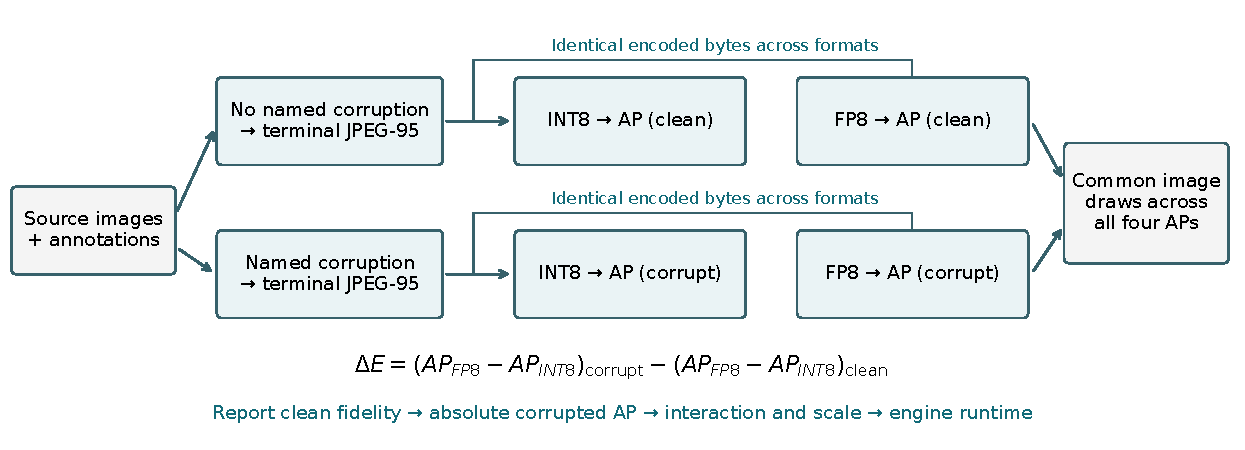
\includegraphics[width=\textwidth]{fig_framework.pdf}
\caption{Paired four-arm evaluation used in the exploratory grid. Clean and corrupted inputs are materialized before the precision branch, and identical encoded bytes are supplied to INT8 and FP8 within each condition. The clean FP8--INT8 gap is subtracted from the corrupted gap inside common image-bootstrap draws to obtain the primary interaction. Original-source clean inputs are used in the final VOC/KITTI holdout; the original/JPEG-95 clean-control substitution is evaluated in a controlled follow-up with fixed engines and one runner.}
\label{fig:framework}
\end{figure*}

\subsection{Paired estimands and reporting order}
\label{sec:estimands}

Let $d$, $m$, $b$, and $c$ index dataset, model, size endpoint, and corruption condition. The exploratory matched-clean control, denoted $\Jclean$, is the source image after deterministic JPEG quality-95 encoding with chroma subsampling disabled and no named corruption. The final holdout replaces $\Jclean$ by original-source clean. AP is evaluated on the $[0,1]$ scale and reported here in AP points after multiplication by 100.

For clean or corrupted input $x$, the direct FP8--INT8 gap is defined as
\begin{equation}
G_{d,m,b,x}=\AP_{d,m,\mathrm{FP8},b,x}-\AP_{d,m,\mathrm{INT8},b,x}.
\end{equation}
The primary interaction is
\begin{align}
\Delta E_{d,m,b,c}=G_{d,m,b,c}-G_{d,m,b,\Jclean}.
\label{eq:delta-e}
\end{align}
For the final holdout, original-source clean replaces $\Jclean$ in Eq.~\eqref{eq:delta-e}. Positive $\Delta E$ means that the signed FP8--INT8 gap is larger after corruption; negative $\Delta E$ means that it is smaller. The contrast is descriptive and conditional on the fixed treatments; it is not a causal difference-in-differences estimator. The FP32 reference cancels algebraically from this direct contrast and is retained only for treatment-verification and reference-relative diagnostics.

Absolute performance is reported separately. For treatment $p$,
\begin{equation}
D_{d,m,p,b,c}=\AP_{d,m,p,b,\Jclean}-\AP_{d,m,p,b,c},
\label{eq:d}
\end{equation}
so $\Delta E=D_{\mathrm{INT8}}-D_{\mathrm{FP8}}$. A negative interaction can therefore arise when FP8 loses more of an initial clean advantage while still retaining higher corrupted AP. It can also occur when both treatments fail: if both corrupted AP values approach zero while the clean gap is fixed,
\begin{equation}
\lim_{\AP_{\mathrm{INT8},c},\AP_{\mathrm{FP8},c}\to0}\Delta E=-G_{\Jclean}.
\label{eq:floor-limit}
\end{equation}
For this reason, corrupted AP and signed loss $D$ are an \emph{absolute-accuracy guardrail}, not a statistical floor test or deployment threshold.

As a secondary scale sensitivity, each treatment's relative retention is
\begin{equation}
R_{d,m,q,b,c}=100\frac{\AP_{d,m,q,b,c}}{\AP_{d,m,q,b,\Jclean}},\qquad
\Delta R=R_{\mathrm{FP8}}-R_{\mathrm{INT8}}.
\label{eq:delta-r}
\end{equation}
$\Delta R$ is reported in percentage points and changes the estimand by normalizing each treatment to its own clean AP. Size-specific interactions are secondary and are detailed in S1; COCO/VOC/KITTI area endpoints and TT100K height endpoints are never pooled.

The interpretation order used throughout the paper is defined in Table~\ref{tab:measurement-contract}. Clean fidelity is checked first, then remaining corrupted accuracy, then the clean-adjusted interaction and its scale sensitivity. Engine efficiency is interpreted only after these accuracy diagnostics.

\begin{table*}[t]
\centering
\caption{Measurement contract for a paired quantized-detector comparison.}
\label{tab:measurement-contract}
\small
\setlength{\tabcolsep}{4pt}
\renewcommand{\arraystretch}{1.16}
\begin{tabular}{Y{2.7cm}Y{3.0cm}Y{4.3cm}Y{4.1cm}}
\toprule
Question & Quantity & What it isolates & Interpretation boundary\\
\midrule
Clean treatment fidelity & $G_{\mathrm{clean}}$ and reference gaps & Difference before the named corruption & Does not measure corruption sensitivity\\
Remaining task performance & $\AP_c$ and $D$ & Corrupted accuracy and clean-to-corrupted loss & Application usefulness needs an external tolerance\\
Change in treatment gap & $\Delta E=G_c-G_{\mathrm{clean}}$ & Corruption-associated change after removing the clean gap & Not a universal format ranking\\
Scale sensitivity & $\Delta R$ & Difference in fractions of clean AP retained & A different denominator-dependent estimand\\
Efficiency & Engine size, latency, throughput & Cost of the recorded executable treatment & Engine-only timing is not end-to-end latency\\
\bottomrule
\end{tabular}
\end{table*}

\subsection{Evidence layers, datasets, and holdout design}
\label{sec:evidence-layers}
\label{sec:datasets}
\label{sec:training}

The exploratory grid contains $4$ datasets $\times3$ YOLO11 capacities $\times4$ corruptions $\times3$ severities $=144$ all-object interaction cells. Its balanced summary is the arithmetic mean over this finite grid, not an estimate weighted for an unspecified deployment population. COCO uses val2017~\citep{lin2014coco}; the transfer datasets use PASCAL VOC~\citep{everingham2015voc}, KITTI~\citep{geiger2012kitti}, and TT100K~\citep{zhu2016tt100k}. VOC and KITTI annotations are converted to the COCO evaluator, so the reported AP values are COCO-style measurements rather than official VOC/KITTI challenge scores. Dataset counts are shown in Table~\ref{tab:datasets}; S1 gives size-endpoint conventions and conversion details.

\begin{table*}[t]
\centering
\caption{Evaluation datasets in the exploratory grid, not the separate final holdouts. Counts are taken from the converted annotations consumed by the evaluator.}
\label{tab:datasets}
\small
\setlength{\tabcolsep}{3pt}
\renewcommand{\arraystretch}{1.18}
\begin{tabular*}{\textwidth}{@{\extracolsep{\fill}}llrrrcl@{}}
\toprule
Dataset & Evaluation split & Images & Objects & \shortstack{Classes\\declared/observed} & \shortstack{Input side\\(pixels)} & Size endpoint \\
\midrule
COCO & val2017 & 5,000 & 36,781 & 80/80 & 640 & Area \\
VOC & VOC2007 test & 4,952 & 12,032 & 20/20 & 640 & Area \\
KITTI & validation & 1,496 & 8,128 & 8/8 & 640 & Area \\
TT100K & test & 3,067 & 8,181 & 221/136 & 1280 & Height \\
\bottomrule
\end{tabular*}
\par\vspace{4pt}\begin{minipage}{\textwidth}\footnotesize
\textit{Size definitions.} Area strata for COCO/VOC/KITTI are $[0,32^2]$, $[32^2,96^2]$, and $\geq96^2$ pixels squared. Original-height strata XS/S/M/L/XL are used for TT100K. Exact endpoint operators are given in S1; area and height endpoints are not pooled.
\end{minipage}

\end{table*}

The historical four-dataset grid is treated as exploratory because VOC2007 test and the recorded KITTI validation partition were used in checkpoint selection. New partitions are frozen for the final rerun before retraining with seed 20260818. For VOC, 8,218 train2007+train2012 images are used for training, 2,510 val2007 images for selection, and 5,823 val2012 images for final evaluation. For KITTI, 1,496 images are reserved for selection, followed by a deterministic label-aware 20\% subset of the remaining images for final evaluation (1,197); the other 4,788 images are used for training. Only training data are used for calibration. The final images are excluded from checkpoint selection, although KITTI scene/drive disjointness is not verified. The paper's strongest post-selection evidence is provided by the resulting six dataset--model blocks and 72 corruption cells.

Original-source clean bytes are used for the final holdout. Because the JPEG-95 matched-clean control is used for the exploratory grid, slightly different clean-control targets are estimated by the two evidence layers. Original-source and JPEG-95 clean images are therefore evaluated in a controlled follow-up with the same retained engine and runner in the six holdout blocks, plus two separately reported TT100K diagnostics. The clean-control substitution is isolated within the recorded execution path; codec equivalence is not established.

\subsection{Precision treatments, corruptions, and execution controls}
\label{sec:precision-treatments}
\label{sec:corruptions}
\label{sec:controlled-clean}

Engines are built with TensorRT 11.1.0.106~\citep{nvidia2026tensorrt} on an RTX 5090 with a 4096 MiB builder workspace. The recorded INT8 and FP8 quantization pipelines are provided by ModelOpt~\citep{nvidia2026modelopt}. TF32 is explicitly disabled for the final high-precision reference; source/ONNX Runtime/FP32 TensorRT agreement is gated at 0.1 AP point and FP32/FP16 TensorRT agreement at 1.0 AP point. These checks are used for consistency rather than as numerical-equivalence proofs. Artifact verification is graded: retained hashes, Q/DQ graph evidence, build records, engine/prediction bindings, and unrecorded fields are reported separately in S1. Graph structure is described by Q/DQ counts; runtime-kernel precision percentages are not inferred from them.

Severity labels 1/3/5 are assigned within the four corruption families: Gaussian noise ($\sigma=8/20/40$ on the 0--255 scale), motion blur (5/13/23-pixel kernels), fog (strength--radius pairs $(0.18,6)/(0.38,12)/(0.62,20)$), and JPEG quality 70/40/15. Deterministic terminal JPEG-95 encoding is applied to exploratory corrupted images and their matched-clean controls with chroma subsampling disabled. Images are materialized once before inference with dimensions and ordered identifiers preserved. Fixed letterbox geometry, confidence $10^{-3}$, class-wise NMS IoU 0.7, a 300-detection decoder cap, and COCOeval \texttt{maxDets}=100 are used for YOLO evaluation.

For the controlled clean-input experiment, original-source and JPEG-95 clean images are passed through the same engine, preprocessing, decoder, threshold, NMS, annotations, class map, and ordered image list. For each block, the control-induced change in the interaction is $S=\Delta E_{\mathrm{J95}}-\Delta E_{\mathrm{original}}=G_{\mathrm{original}}-G_{\mathrm{J95}}$ while the corrupted arms are held fixed. One estimate is reported per block; reusing the same clean gap across multiple corruptions is not treated as repeated codec evidence.

\subsection{AP evaluation and paired uncertainty}
\label{sec:uncertainty}

AP is evaluated over IoU thresholds 0.50--0.95. The image is used as the resampling unit~\citep{efron1979bootstrap}. Within each dataset and evidence layer, one deterministic schedule of 2,000 image-index bootstrap draws is reused across the related clean, corrupted, INT8, and FP8 arms. Per-image COCOeval entries are indexed by the sampled position list in the custom AP accumulator without deduplication; duplicate image IDs are not passed back to \texttt{COCOeval.evaluate()}. Tie order is preserved through stable score sorting, and the interaction is calculated inside each common draw before aggregation. The observed covariance between the clean and corrupted treatment gaps is preserved by the shared schedule.

Uncertainty from the finite evaluation images is therefore quantified by percentile intervals conditional on fixed checkpoints, calibration lists, engines, corruptions, decoding, and evaluation splits. Training-seed, calibration-seed, engine-build, dataset-selection, and corruption-population uncertainty are not propagated, and individual-cell intervals are not multiplicity-adjusted. Possible within-scene dependence is not accounted for by image resampling; KITTI scene/drive independence was not verified. The raw corrupted gap $G_c$ is compared with $\Delta E$ in the point-sign diagnostic; a sign disagreement is interpreted as a change of estimand, not as two contradictory statistical decisions. In a retained-draw covariance audit, the paired variance is compared with the variance obtained after analytically removing only the observed clean--corrupted gap covariance. A fixed-class-universe Bayesian-bootstrap sensitivity for TT100K is also reported in S1~\citep{rubin1981bayesian}.

\subsection{Sensitivity analyses and secondary diagnostics}
\label{sec:sensitivities}
\label{sec:crossfamily-methods}
\label{sec:attachment-method}

Three targeted analyses probe conditionality beyond finite-image resampling. First, YOLO11m is evaluated on frozen, label-aware 512-image subsets of VOC, KITTI, and TT100K under three fixed corruption labels; stochastic fields and blur angles are nested across severity in this sensitivity, whereas deterministic JPEG repeats across labels. Second, a $3\times3$ crossing of training and calibration seeds is evaluated for YOLO11m on the same transfer datasets at severity 5. Third, the 144-cell ledger is re-aggregated with image-count and object-count weights and after omitting each dataset or corruption family. These are bounded design sensitivities, not repeated estimates of one population parameter~\citep{bouthillier2021variance}.

RT-DETR-L~\citep{carion2020detr,zhao2024rtdetr} and RetinaNet~\citep{lin2017focal,torchvision2026retinanet} are retained as quantization-recipe portability stress tests. Their transferred INT8 treatments lose substantial clean accuracy, so these blocks are not used as balanced cross-family FP8--INT8 comparisons. A build-policy-matched default-versus-aligned INT8 comparison in KITTI--RetinaNet, which reuses rather than rebuilds FP8, and TIDE AP50 diagnostics~\citep{bolya2020tide} are reported in S1 as secondary evidence, not mechanistic explanations of datatype behavior.

\subsection{AI-assisted research workflow}

OpenAI Codex was used as an author-supervised coding assistant for parts of experimental orchestration, analysis implementation, validation, and consistency checking. The hosted model snapshot was not retained in the historical experiment records. AI-generated code or suggestions were reviewed, tested, and edited by the authors; detector predictions and numerical measurements were produced by the recorded experimental software rather than by a generative-AI model. Use of generative AI for manuscript preparation is disclosed separately at the end of the article.

\section{Results}
\label{sec:results}

\subsection{Primary selection-disjoint holdout evidence}
\label{sec:protocol-check}
\label{sec:holdout-results}

AP is recomputed from annotations and predictions by the delivered four-arm evaluator without reliance on AP caches. Zero interaction for identical treatments or identical clean/corrupted predictions, sign reversal after treatment exchange, repeated-image multiplicity, and rejection of mismatched image or execution settings are verified with regression fixtures.

\begin{samepage}
In a prediction-level worked example using KITTI's 1,197 final images with YOLO11m and fog severity 1, clean INT8/FP8 AP of 67.3281/70.5287 and corrupted AP of 63.5892/66.5094 are reproduced. A 2.9202 AP advantage is therefore retained by FP8 under corruption, but the clean gap of 3.2007 AP is reduced, yielding $\Delta E=-0.2805$ AP. An interval of $[-1.2692,+0.7844]$ is regenerated from 2,000 draws.
\end{samepage}

Across all six final VOC/KITTI dataset--model blocks, FP8's original-clean advantage averages 1.60 AP points and is positive in every block. Under corruption, the balanced FP8--INT8 gap remains positive at $+1.05$ AP with a paired 95\% percentile interval of $[+0.91,+1.16]$. The clean-adjusted interaction, however, is $-0.55$ AP $[-0.78,-0.29]$. Dataset means are $-0.43$ AP for VOC and $-0.67$ AP for KITTI (Table~\ref{tab:holdout}). Thus the strongest holdout result is not that FP8 becomes worse under corruption; it is that a positive absolute advantage becomes smaller after accounting for the advantage already present on clean images.

All six strict high-precision reference-parity blocks passed. The largest source-to-FP32-engine difference was 0.0404 AP and the largest FP32-to-FP16 difference was 0.2554 AP. Figure~\ref{fig:holdout-primary} keeps the final holdout separate from the historical and four-dataset exploratory summaries because their partitions, checkpoint histories, and clean-control definitions differ.

\begin{figure}[pos=t]
\centering
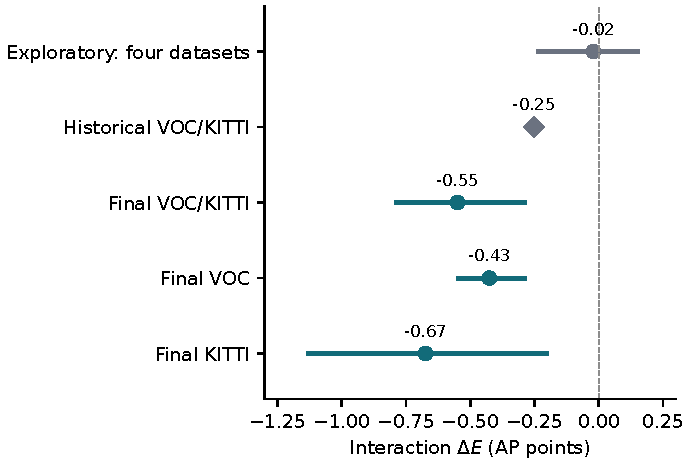
\includegraphics[width=\columnwidth]{fig_holdout_primary.pdf}
\caption{Selection-disjoint VOC/KITTI holdout evidence beside historical and exploratory context. Bars are paired-image percentile intervals within each stated scope; the historical two-dataset value is shown only as a contextual point estimate.}
\label{fig:holdout-primary}
\end{figure}

\begin{table}[t]
\centering
\caption{Dataset summaries from the final holdouts using original-source clean controls. Effects and intervals are AP points from common paired image samples.}
\label{tab:holdout}
\small
\setlength{\tabcolsep}{2pt}
\renewcommand{\arraystretch}{1.18}
\begin{tabular}{@{}lrrrrc@{}}
\toprule
Dataset & \shortstack{Selection\\images} & \shortstack{Final\\images} & Cells & \shortstack{Mean\\$\Delta E$} & \shortstack{95\%\\interval} \\
\midrule
VOC & 2,510 & 5,823 & 36 & -0.43 & $[-0.54,-0.29]$ \\
KITTI & 1,496 & 1,197 & 36 & -0.67 & $[-1.13,-0.20]$ \\
\bottomrule
\end{tabular}
\end{table}

The four AP components behind this interpretation are reported in Panel A of Table~\ref{tab:v4_holdout_four_ap}; the corresponding gaps and intervals are separated in Panel B. A positive corrupted gap and a negative interaction must not be read as contradictory rankings: the former is measured against INT8 on corrupted images, whereas the latter is measured against the pre-existing clean gap. In a post hoc point-sign diagnostic of the frozen holdout grid, 52 positive raw corrupted gaps are identified; 29 negative point estimates are obtained after clean adjustment. Eight of those adjusted intervals are entirely below zero and zero is included in the other 21. These counts are used to describe changes in the estimand and are not interpreted as multiplicity-adjusted discoveries.

% Generated by analysis/build_v4_publication_tables.py; do not edit.
\begin{table*}[tp]
\centering
\small
\setlength{\tabcolsep}{3pt}
\renewcommand{\arraystretch}{1.22}
\caption{Selection-disjoint holdout results with original-source clean controls. Absolute AP is shown in Panel A; the corresponding gaps and paired uncertainty are shown in Panel B. All values are AP points.}
\label{tab:v4_holdout_four_ap}
\begin{tabular*}{\textwidth}{@{\extracolsep{\fill}}llrrrr@{}}
\toprule
\multicolumn{6}{@{}l}{\textbf{A. Absolute task accuracy}} \\
\addlinespace[3pt]
 & & \multicolumn{2}{c}{Original clean AP} & \multicolumn{2}{c}{Mean corrupted AP} \\
\cmidrule(lr){3-4}\cmidrule(lr){5-6}
Dataset & Model & INT8 & FP8 & INT8 & FP8 \\
\midrule
VOC & YOLO11n & 53.41 & 53.84 & 37.13 & 37.69 \\
VOC & YOLO11m & 56.26 & 57.91 & 40.34 & 41.19 \\
VOC & YOLO11x & 58.43 & 58.66 & 42.64 & 42.27 \\
\addlinespace[4pt]
KITTI & YOLO11n & 58.33 & 60.53 & 41.12 & 42.44 \\
KITTI & YOLO11m & 67.33 & 70.53 & 46.00 & 48.14 \\
KITTI & YOLO11x & 68.90 & 70.80 & 46.74 & 48.55 \\
\bottomrule
\end{tabular*}
\par\vspace{9pt}
\begin{tabular*}{\textwidth}{@{\extracolsep{\fill}}llrrcrc@{}}
\toprule
\multicolumn{7}{@{}l}{\textbf{B. FP8--INT8 gaps and clean-adjusted interaction}} \\
\addlinespace[3pt]
Dataset & Model & \shortstack{Clean gap\\$G_0$} & \shortstack{Corrupted gap\\$G_c$} & \shortstack{95\% interval\\for $G_c$} & \shortstack{Interaction\\$\Delta E$} & \shortstack{95\% interval\\for $\Delta E$} \\
\midrule
VOC & YOLO11n & +0.4274 & +0.5610 & [0.4368, 0.6855] & +0.1336 & [-0.0757, 0.3982] \\
VOC & YOLO11m & +1.6546 & +0.8498 & [0.6888, 0.9554] & -0.8048 & [-1.0208, -0.5717] \\
VOC & YOLO11x & +0.2291 & -0.3762 & [-0.4762, -0.2808] & -0.6053 & [-0.7919, -0.4096] \\
\addlinespace[4pt]
KITTI & YOLO11n & +2.1946 & +1.3196 & [0.9552, 1.7035] & -0.8750 & [-1.7850, 0.0994] \\
KITTI & YOLO11m & +3.2007 & +2.1344 & [1.7440, 2.4366] & -1.0662 & [-1.9657, -0.1723] \\
KITTI & YOLO11x & +1.8938 & +1.8128 & [1.4292, 2.1585] & -0.0810 & [-0.8485, 0.5881] \\
\midrule
\multicolumn{3}{@{}l}{\textbf{Equal-block mean (six blocks)}} & +1.0502 & [0.9105, 1.1554] & -0.5498 & [-0.7843, -0.2908] \\
\bottomrule
\end{tabular*}
\par\vspace{5pt}\begin{minipage}{\textwidth}\footnotesize
\textit{How to read the table.} A positive $G_c$ denotes higher corrupted AP for FP8; a negative $\Delta E$ denotes a smaller signed gap than on clean inputs. Thus higher corrupted accuracy and a contracting advantage can be observed together.
\par\smallskip\textit{Definitions.} $G_0=A_{F,0}-A_{I,0}$, $G_c=\overline{A}_{F,c}-\overline{A}_{I,c}$, and $\Delta E=G_c-G_0$. Corrupted AP is averaged equally over twelve corruption--severity cells per block. Contrasts are computed from unrounded AP, not from the two-decimal values in Panel A.
\par\smallskip\textit{Uncertainty and provenance.} Paired 95\% percentile intervals are based on 2,000 draws; block and macro means are formed before percentiles are taken. The $G_c$ intervals are reconstructed from retained $\Delta E$ draws and original-clean AP draws on the recorded historical schedule. Historical NumPy/evaluator versions were not recorded. These estimates are not terminal-codec matched; recovery details are provided in S1.
\end{minipage}
\end{table*}


\subsection{Clean-control sensitivity and absolute corrupted accuracy}
\label{sec:controlled-clean-results}
\label{sec:clean-results}
\label{sec:absolute-results}

The controlled clean-input follow-up completed all 32 clean arms with fixed engines and execution settings. Across the six final-holdout blocks, replacing original-source clean by JPEG-95 clean changes the interaction by only $+0.0574$ AP on average, with paired interval $[-0.1839,+0.2518]$. Individual point shifts range from $-0.2902$ to $+0.7985$ AP and all six intervals cross zero (Table~\ref{tab:v4_clean_control}). The separately selected TT100K n/x diagnostics have larger point shifts ($+0.8995$ and $+1.1878$ AP) but wide intervals that also cross zero. The experiment therefore reduces concern that the six-block holdout result is driven by the clean codec choice, while providing no equivalence claim for codecs in general.

% Generated by analysis/build_v4_publication_tables.py; do not edit.
\begin{table*}[tp]
\centering
\small
\setlength{\tabcolsep}{3pt}
\renewcommand{\arraystretch}{1.18}
\caption{Effect of replacing original-source clean inputs with JPEG-95 clean controls. All values are AP points; engines and image draws are held fixed.}
\label{tab:v4_clean_control}
\begin{tabular*}{\textwidth}{@{\extracolsep{\fill}}llrrrrrc@{}}
\toprule
 & & \multicolumn{2}{c}{Original clean} & \multicolumn{2}{c}{JPEG-Q95 clean} & & \\
\cmidrule(lr){3-4}\cmidrule(lr){5-6}
Dataset & Model & INT8 & FP8 & INT8 & FP8 & Shift $S$ & 95\% interval \\
\midrule
\multicolumn{8}{@{}l}{\textbf{Primary: six VOC/KITTI holdout blocks}} \\
\addlinespace[2pt]
VOC & YOLO11n & 53.41 & 53.84 & 53.32 & 53.75 & +0.0011 & [-0.2693, 0.2324] \\
VOC & YOLO11m & 56.26 & 57.91 & 56.04 & 57.74 & -0.0460 & [-0.2434, 0.1774] \\
VOC & YOLO11x & 58.43 & 58.66 & 58.26 & 58.59 & -0.1011 & [-0.3000, 0.0561] \\
\addlinespace[4pt]
KITTI & YOLO11n & 58.33 & 60.53 & 58.40 & 60.61 & -0.0182 & [-0.8572, 0.9690] \\
KITTI & YOLO11m & 67.33 & 70.53 & 67.80 & 70.20 & +0.7985 & [-0.0440, 1.5560] \\
KITTI & YOLO11x & 68.90 & 70.80 & 68.61 & 70.79 & -0.2902 & [-0.9880, 0.4470] \\
\midrule
\multicolumn{6}{@{}l}{\textbf{Primary equal-block mean}} & +0.0574 & [-0.1839, 0.2518] \\
\midrule
\multicolumn{8}{@{}l}{\textbf{Diagnostic: TT100K (not pooled)}} \\
\addlinespace[2pt]
TT100K & YOLO11n & 25.10 & 27.12 & 25.29 & 26.41 & +0.8995 & [-0.1497, 1.9384] \\
TT100K & YOLO11x & 55.50 & 56.76 & 56.02 & 56.10 & +1.1878 & [-0.7891, 2.1028] \\
\bottomrule
\end{tabular*}
\par\vspace{4pt}\begin{minipage}{\textwidth}\footnotesize
\textit{Reading the shift.} $S=G_{\mathrm{original}}-G_{\mathrm{J95}}=\Delta E_{\mathrm{J95}}-\Delta E_{\mathrm{original}}$, with corrupted predictions held fixed. A positive value denotes a larger interaction after clean-control substitution, not improved corrupted accuracy. One estimate is reported per block.
\par\smallskip\textit{Uncertainty.} Paired-image percentile intervals are based on 2,000 draws, conditional on retained engines and encoded bytes. The primary mean is formed within each draw before percentiles are taken; TT100K diagnostics are excluded. Contrasts are computed from unrounded AP.
\end{minipage}
\end{table*}


In the exploratory grid, FP8 has higher JPEG-95 clean AP than INT8 in all 12 dataset--YOLO combinations, by 1.40 AP on average. Under corruption, 282 of 288 treatment arms lose AP relative to their matched-clean input; the median signed loss is 5.51 AP and the mean is 15.24 AP. Thirty-five exploratory arms fall below the descriptive guide of 10 AP and nine fall below 5 AP. These values are not deployment thresholds. They establish why a clean-adjusted interaction cannot substitute for reporting remaining task accuracy: a shrinking treatment gap can occur even when both detectors perform poorly. Dataset-level absolute summaries are shown in Table~\ref{tab:absolute-guardrail}.

\begin{table*}[t]
\centering
\caption{Absolute corrupted-accuracy guardrail from the exploratory YOLO ledger. The signed loss is $D=\AP_{\Jclean}-\AP_c$. Rows are balanced descriptive summaries, not deployment thresholds or pooled leaderboard scores.}
\label{tab:absolute-guardrail}
\small
\setlength{\tabcolsep}{4pt}
\renewcommand{\arraystretch}{1.18}
\begin{tabular*}{\textwidth}{@{\extracolsep{\fill}}llrrrrr@{}}
\toprule
 & & & \multicolumn{2}{c}{All corruptions} & \multicolumn{2}{c}{Severity 5 only} \\
\cmidrule(lr){4-5}\cmidrule(lr){6-7}
Dataset & Format & Clean AP & Mean AP & Mean loss $D$ & Mean AP & Mean loss $D$ \\
\midrule
COCO & INT8 & 46.010 & 34.911 & 11.099 & 25.185 & 20.826 \\
COCO & FP8 & 47.110 & 35.824 & 11.286 & 25.667 & 21.443 \\
\addlinespace[4pt]
VOC & INT8 & 65.732 & 49.246 & 16.486 & 35.478 & 30.255 \\
VOC & FP8 & 66.828 & 50.300 & 16.529 & 36.023 & 30.805 \\
\addlinespace[4pt]
KITTI & INT8 & 67.284 & 46.445 & 20.839 & 29.881 & 37.403 \\
KITTI & FP8 & 69.797 & 48.498 & 21.299 & 31.504 & 38.293 \\
\addlinespace[4pt]
TT100K & INT8 & 44.760 & 32.270 & 12.490 & 22.573 & 22.188 \\
TT100K & FP8 & 45.636 & 33.752 & 11.884 & 23.467 & 22.169 \\
\bottomrule
\end{tabular*}

\end{table*}

\subsection{Exploratory landscape and decision impact}
\label{sec:decision-impact}
\label{sec:exploratory-results}

Across the 144 exploratory cells, the raw corrupted FP8--INT8 gap is positive in 134 cells and averages 1.38 AP. The 12 dataset--model clean gaps are also all positive and average 1.40 AP. After subtracting the matched-clean gap, mean $\Delta E$ is $-0.02$ AP and the point estimates split into 78 positive and 66 negative values. Fifty-six cells change from a positive raw gap to a negative clean-adjusted point estimate (Fig.~\ref{fig:decision-impact}A); 17 of their adjusted intervals lie entirely below zero and 39 cross zero. Twenty-two of the 56 disagreements have $|\Delta E|<0.25$ AP and 36 have $|\Delta E|<0.50$ AP, so the sign count should not be interpreted as 56 practically large reversals.

Figure~\ref{fig:decision-impact}B adds the lower corrupted AP of the two treatments. Eighteen cells have at least one treatment below 10 AP and five have at least one below 5 AP. This visualization makes the two required questions explicit: clean adjustment changes the comparison target, while absolute AP determines whether the remaining detector performance is meaningful for a particular application.

\begin{figure*}[t]
\centering
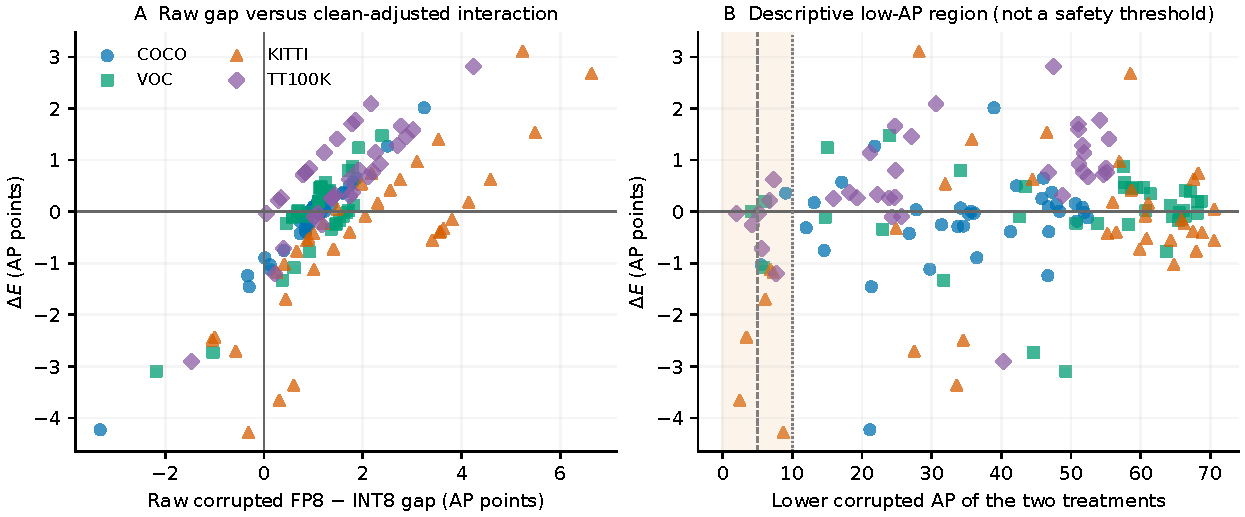
\includegraphics[width=\textwidth]{fig_decision_impact.pdf}
\caption{Why raw corrupted superiority and clean-adjusted sensitivity can differ. (A) The raw corrupted FP8--INT8 gap includes the pre-existing clean gap. (B) The same interaction values are shown against the lower corrupted AP of the two treatments; 5- and 10-AP lines are descriptive guides rather than deployment thresholds.}
\label{fig:decision-impact}
\end{figure*}

The balanced four-dataset mean $\overline{\Delta E}_{\mathrm{grid}}$ is $-0.02$ AP with percentile interval $[-0.24,+0.15]$, but condition-level effects are heterogeneous: they range from $-4.28$ to $+3.10$ AP. Dataset means span $-0.46$ AP for KITTI to $+0.61$ AP for TT100K (Table~\ref{tab:dataset-margins}). The near-zero macro therefore does not imply that individual conditions are insensitive to corruption or that a single format dominates across datasets.

\begin{table}[t]
\centering
\caption{All-object dataset summaries from the exploratory paired ledger.}
\label{tab:dataset-margins}
\small
\begin{tabular}{lrr}
\toprule
Dataset & Cells & Mean $\Delta E$\\
\midrule
COCO & 36 & -0.19\\
VOC & 36 & -0.04\\
KITTI & 36 & -0.46\\
TT100K & 36 & +0.61\\
\bottomrule
\end{tabular}
\end{table}

\begin{figure*}[t]
\centering
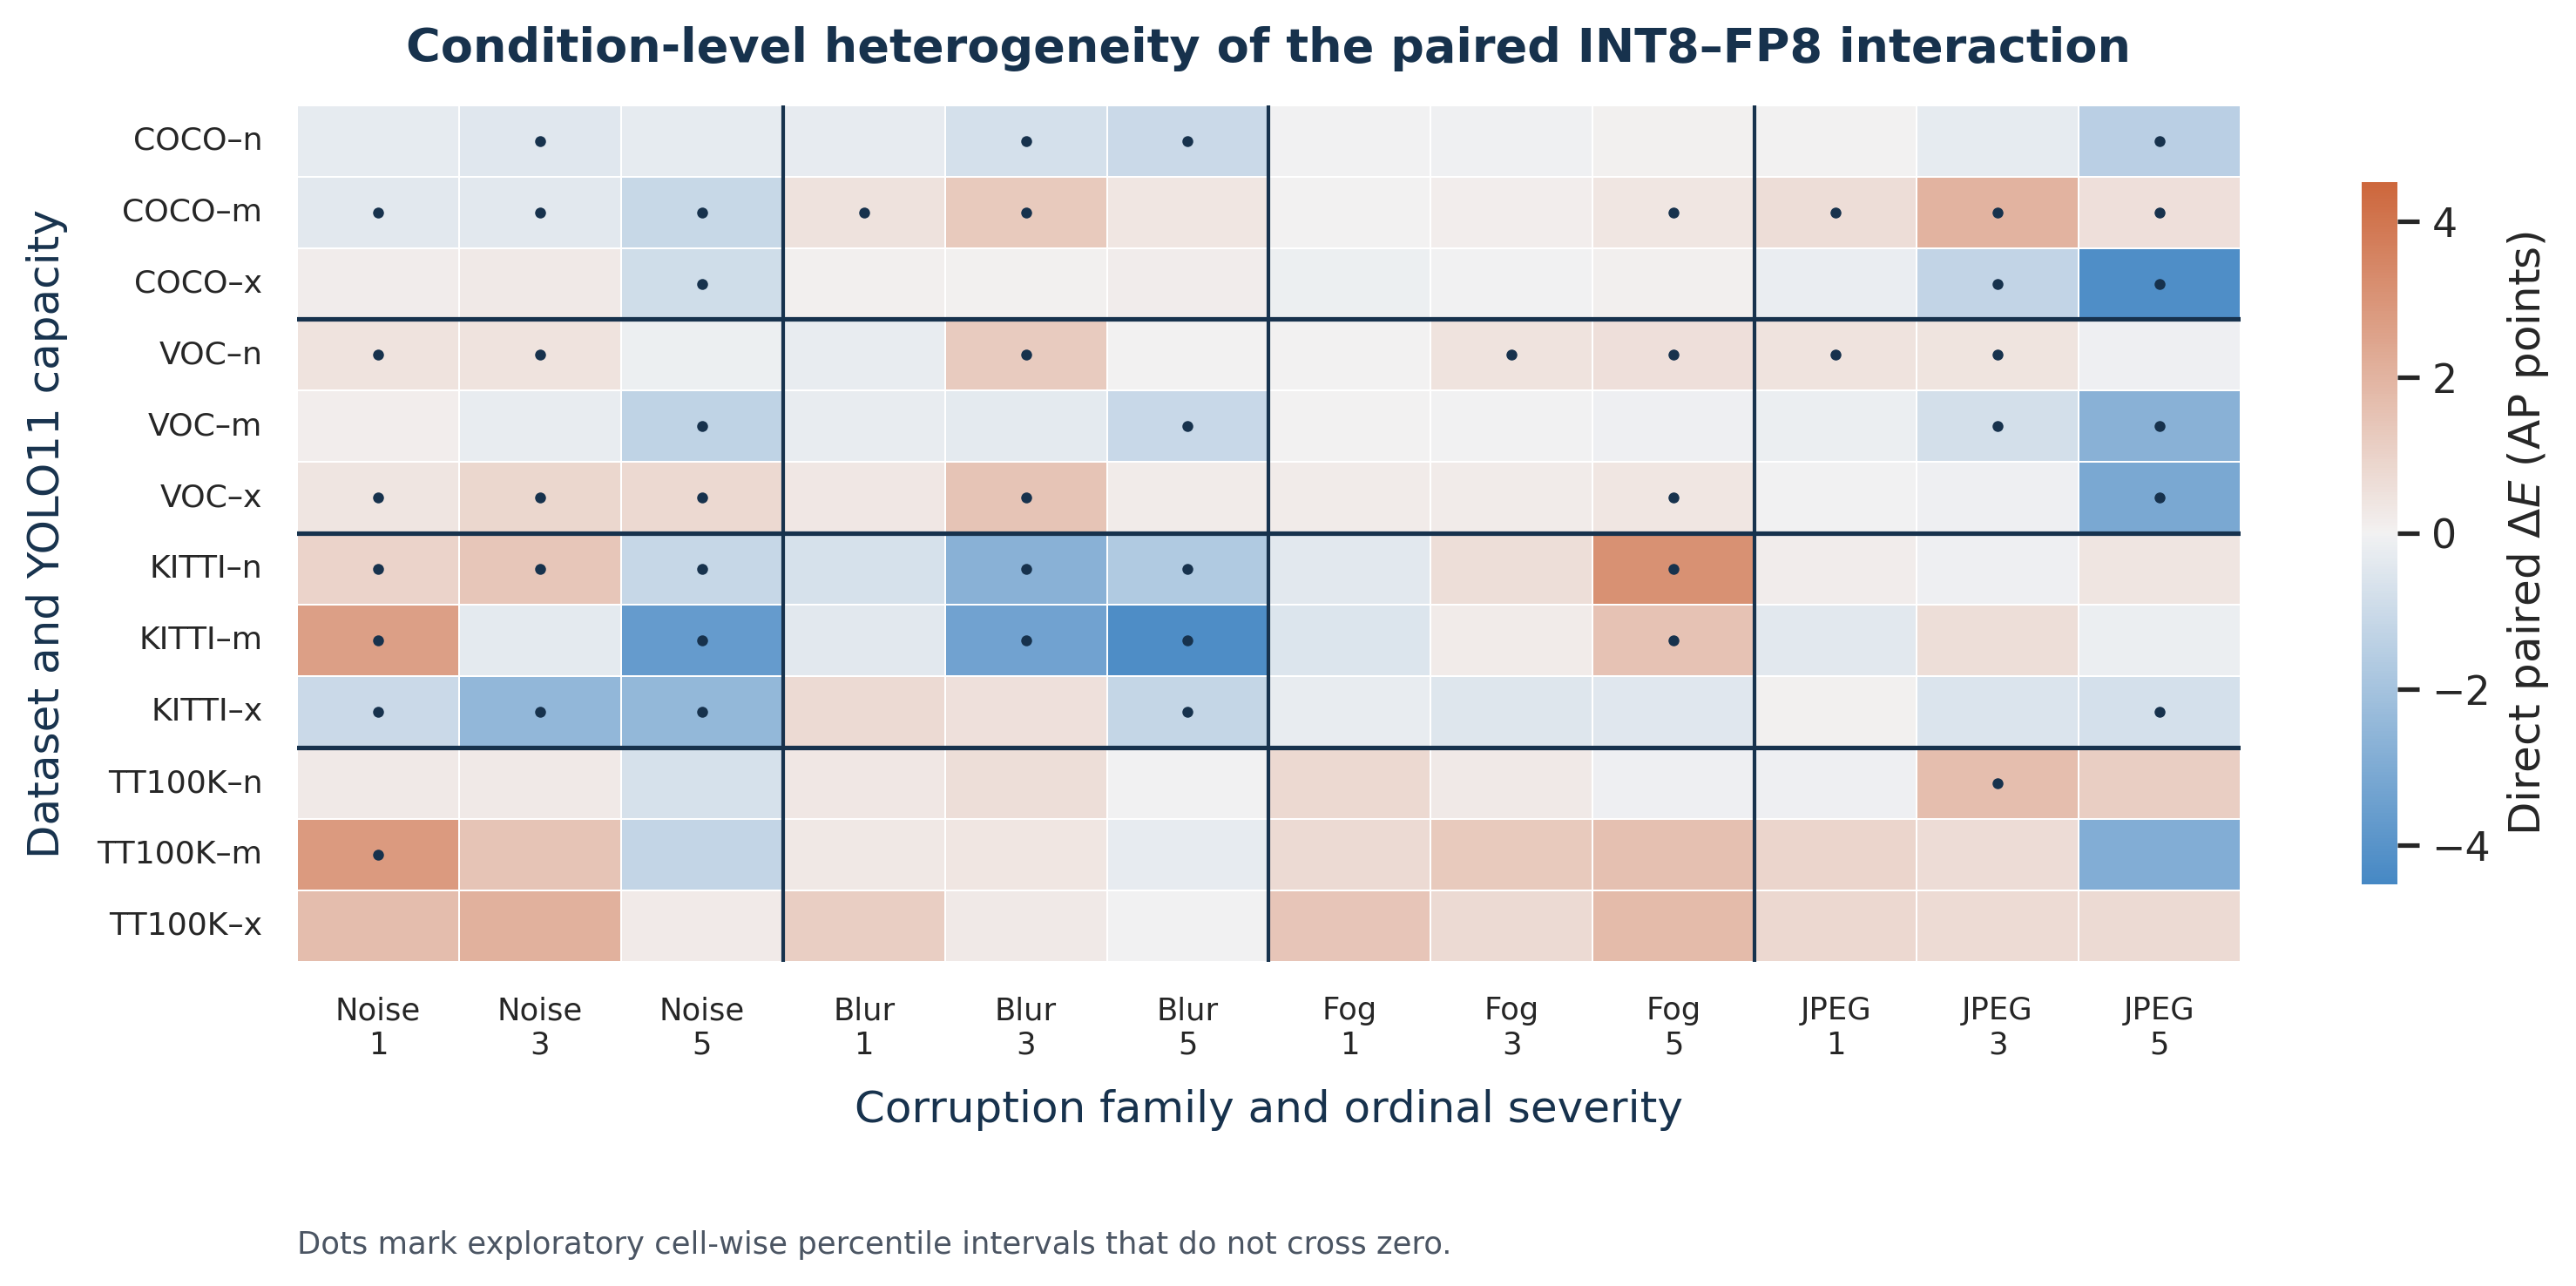
\includegraphics[width=\textwidth]{fig_direct_heterogeneity_heatmap.png}
\caption{Exploratory interaction heterogeneity across dataset, YOLO11 capacity, corruption, and severity. Dots mark individual-cell percentile intervals that do not cross zero; these intervals are exploratory and are not adjusted for multiple comparisons.}
\label{fig:heterogeneity}
\end{figure*}

\subsection{Sensitivity to estimand, pairing, and design choices}
\label{sec:component-results}
\label{sec:scale-results}
\label{sec:covariance-results}
\label{sec:sensitivity-results}

Table~\ref{tab:components} summarizes the main measurement consequences. Clean subtraction changes the estimand and produces the 56/144 exploratory point-sign disagreements above. Preserving clean--corrupted covariance does not change the point estimate, but setting that covariance to zero increases the estimated SD in 127 of 144 cells. The median zero-covariance/paired SD ratio is 1.124 (range 0.912--1.748), showing that shared-image sampling has a measurable and data-dependent effect on uncertainty.

\begin{table*}[t]
\centering\small
\caption{Empirical consequences of key protocol choices. The rows change either the scientific target, the uncertainty calculation, or the reporting context; they are not an algorithmic ablation leaderboard.}
\label{tab:components}
\setlength{\tabcolsep}{4pt}
\renewcommand{\arraystretch}{1.16}
\begin{tabular}{Y{2.7cm}Y{2.7cm}Y{4.5cm}Y{4.3cm}}
\toprule
Component & What changes? & Observed consequence & Interpretation boundary\\
\midrule
Subtract clean gap & Estimand: $G_c$ to $\Delta E$ & 56/144 exploratory point-sign changes & Not 56 multiplicity-adjusted discoveries\\
Preserve clean--corrupted covariance & Uncertainty, not point estimand & Zero-covariance SD larger in 127/144 cells; median ratio 1.124 & Does not establish interval coverage\\
Report absolute corrupted AP & Adds task-performance context & 282/288 exploratory arms lose AP; 35 below 10 AP & Descriptive cutoffs, not estimated failure thresholds\\
Use relative retention & Estimand and scale & 18/144 exploratory and 7/72 holdout sign disagreements with $\Delta E$ & Denominator-dependent sensitivity\\
Clean-control substitution & Clean comparison target & Six-holdout mean shift $+0.057$ AP, interval crosses zero & No general codec-equivalence claim\\
\bottomrule
\end{tabular}
\end{table*}

The relative-retention contrast yields a different scale-dependent summary. Across the exploratory grid, mean $\Delta E$ is $-0.02$ AP whereas mean $\Delta R$ is $+0.75$ percentage points, with 18 cell-level sign disagreements. Across the final holdouts, the corresponding means are $-0.55$ AP and $-0.12$ percentage points, with seven sign disagreements. KITTI's final dataset mean changes from $-0.67$ AP on the additive scale to $+0.10$ percentage points on the retention scale. $\Delta E$ is retained as the primary estimand because it directly answers how the between-treatment AP-point gap changes; $\Delta R$ answers how much of each treatment's own clean AP is retained.

\begin{table*}[t]
\centering
\caption{Metric-scale sensitivity, with scope-wide summaries separated from dataset rows. $\Delta R$ is the FP8-minus-INT8 difference in the percentage of clean AP retained, using each evidence layer's recorded clean control. Sign differences are counted between cell-level point estimates of $\Delta E$ and $\Delta R$, not between interval-based decisions.}
\label{tab:relative-retention}
\small
\setlength{\tabcolsep}{6pt}
% Generated by analysis/build_cviu_revision_artifacts.py.
\begin{tabular}{lrrrr}
\toprule
Scope & Cells & Mean $\Delta E$ (AP) & Mean $\Delta R$ (pp) & Sign differences \\
\midrule
\textbf{Exploratory grid} & 144 & -0.02 & +0.75 & 18 \\
Exploratory: COCO & 36 & -0.19 & +0.16 & 1 \\
Exploratory: VOC & 36 & -0.04 & +0.35 & 6 \\
Exploratory: KITTI & 36 & -0.46 & +0.49 & 6 \\
Exploratory: TT100K & 36 & +0.61 & +1.98 & 5 \\
\midrule
\textbf{Final holdouts} & 72 & -0.55 & -0.12 & 7 \\
Final: VOC & 36 & -0.43 & -0.34 & 3 \\
Final: KITTI & 36 & -0.67 & +0.10 & 4 \\
\bottomrule
\end{tabular}

\end{table*}

Other design sensitivities support conditional rather than universal interpretation. Equal-, image-count-, and object-count-weighted exploratory means are $-0.02$, $+0.00$, and $-0.09$ AP; leave-one-dataset means range from $-0.23$ to $+0.13$ AP. Three corruption-realization labels produce mean interactions of $-0.12$, $-0.26$, and $-0.32$ AP in their targeted branch. In the $3\times3$ training/calibration seed study, the balanced mean is $-1.11$ AP, with training-seed marginals from $-1.64$ to $-0.68$ and calibration-seed marginals from $-1.32$ to $-0.84$ AP. The TT100K fixed-class-universe bootstrap preserves the negative height-macro direction but changes whether the overall interval crosses zero. Full conditionality tables and Monte Carlo checks are reported in S1.

\subsection{Runtime and cross-family portability stress tests}
\label{sec:runtime-results}
\label{sec:crossfamily-results}
\label{sec:attachment-results}
\label{sec:tide-results}

Across the 12 corresponding YOLO conditions, the median of the condition-wise FP32/INT8 latency ratios is 2.96$\times$, and the corresponding FP32/FP8 median is 3.13$\times$. The median of the condition-wise INT8/FP8 ratios is 1.08$\times$ with a range of 0.92--1.19$\times$, so FP8 is not faster in every condition. These are engine-only measurements on one RTX 5090 and exclude image decoding, preprocessing, transfer, detector decoding, NMS, power, and energy (Table~\ref{tab:runtime}).

\begin{table}[t]
\centering
\caption{TensorRT engine measurements on the RTX 5090. Values for each condition are medians of three runs; each row summarizes 12 corresponding YOLO conditions.}
\label{tab:runtime}
\small
\setlength{\tabcolsep}{3pt}
\renewcommand{\arraystretch}{1.18}
\begin{tabular}{lrrrr}
\toprule
Precision & $n$ & \shortstack{Size\\(MiB)} & \shortstack{Latency\\(ms)} & \shortstack{Throughput\\(qps)} \\
\midrule
FP32 & 12 & 79.90 & 2.434 & 410.6 \\
INT8 & 12 & 24.07 & 0.789 & 1265.3 \\
FP8 & 12 & 21.92 & 0.760 & 1315.7 \\
\bottomrule
\end{tabular}

\par\vspace{3pt}\begin{minipage}{\columnwidth}\footnotesize
\textit{Reading the ratios.} Matched-condition latency ratios are reported in the text; they are not ratios of the marginal medians shown here. Timing is engine-only.
\end{minipage}
\end{table}

The RT-DETR-L and RetinaNet blocks are not balanced format comparisons. The transferred INT8 recipe has mean clean-reference gaps of 38.66 AP for RT-DETR-L and 22.53 AP for RetinaNet, with mean corrupted AP of only 1.97 and 11.34. A build-policy-matched KITTI--RetinaNet default-versus-aligned INT8 comparison improves aligned INT8 clean AP from 7.13 to 14.83 and mean corrupted AP from 7.43 to 12.07, but remains far from the reused FP8 treatment (49.27 clean AP and 36.48 mean corrupted AP), which was not rebuilt. These experiments demonstrate recipe-portability failure and bound the study's generalization; they do not establish that INT8 is intrinsically less robust than FP8. S1 reports the rebuild contrast and secondary TIDE diagnostics.

\section{Discussion}
\label{sec:discussion}

\subsection{Absolute superiority and corruption sensitivity are different claims}

The final holdout provides the clearest example of the paper's central measurement distinction. FP8 begins 1.60 AP ahead of INT8 on original-clean images and remains 1.05 AP ahead after corruption, yet the clean-adjusted interaction is $-0.55$ AP. There is no contradiction: the absolute corrupted-input comparison favors FP8, while the interaction says that part of its pre-existing advantage is lost under corruption. The same pattern occurs at cell level in both the exploratory and selection-disjoint grids. Reporting only the corrupted gap would hide this change; reporting only the interaction would hide the fact that FP8 still retains higher corrupted AP on average.

The absolute-accuracy guardrail is equally important. Equation~\eqref{eq:floor-limit} shows that when both treatments approach zero corrupted AP, an initially positive clean gap mechanically yields a negative limiting interaction. A negative $\Delta E$ therefore cannot be interpreted as useful robustness without the corrupted AP values themselves. Conversely, relative retention can disagree in sign with the additive AP-point interaction because it normalizes by different clean denominators. These are not competing answers to one metric; they are different estimands and should be named explicitly.

\subsection{What the paired protocol contributes}

The practical contribution is provided by the combination of measurement and execution constraints. The same condition-specific bytes are supplied to INT8 and FP8 through shared inputs; the four AP arms are kept paired through common image draws; the clean control is explicitly defined; and absolute performance is reported before the interaction. A measurable role for the shared resampling schedule is demonstrated by the covariance audit: the estimated SD in most exploratory cells is changed by analytically removing only the observed clean--corrupted covariance. In the prediction-level worked example, the reported effect is linked to an evaluator through which AP and uncertainty are reconstructed from retained predictions rather than from cached aggregate scores.

The controlled clean-input study clarifies another source of ambiguity. In the six final holdout blocks, original-source versus JPEG-95 clean substitution changes the interaction by only about $+0.06$ AP on average and its interval crosses zero. This reduces the weight of the historical codec mismatch as an explanation for the final result, but it does not prove codec invariance. The stronger methodological point is that control substitution can be isolated and estimated rather than left implicit.

\subsection{Implications for evaluating compressed neural networks}

The distinction matters when an improved quantization recipe raises clean accuracy: a larger corrupted-input gap may then reflect better clean fidelity rather than reduced degradation sensitivity. For evaluating a calibration, rounding, or mixed-precision change, the reusable procedure is to freeze both executable candidates, define the same clean control and corrupted inputs, and report their four task scores with paired uncertainty. The application-specific minimum accuracy and cost requirements must be specified separately; the protocol does not supply a universal pass/fail rule. A favorable interaction cannot rescue an unusable corrupted detector, and an unfavorable interaction does not negate a higher absolute corrupted score.

Recipe portability must also be distinguished from robustness. Relevant context for possible off-the-shelf recipe failure on RT-DETR is provided by QRT-DETR's architecture-tailored quantization and reconstruction~\citep{huo2026qrt}. The failure in the retained engines is not diagnosed by that work, and its low-bit results should not be compared directly with this INT8--FP8 study. Before a format comparison is extended to another neural architecture, competitive clean treatments must be established for that architecture. This evaluation discipline is supported by the present evidence for the measured detectors; its utility for other tasks remains to be tested.

\subsection{Scope, generalization, and limitations}

The primary empirical evidence is a YOLO11 TensorRT study. RT-DETR and RetinaNet do not extend the format comparison because their transferred INT8 recipes are not clean-competitive. The RetinaNet follow-up improves aligned INT8 but remains far from the frozen FP8 comparator, showing that matching the two INT8 builds' recorded settings is insufficient for a balanced cross-family comparison. FP8 was not rebuilt under that matched policy. A stronger claim about architecture-independent INT8--FP8 robustness would require clean-competitive treatments for multiple detector families under matched build policies.

The corruption coverage is also bounded. Four synthetic corruption families and three severities do not represent all natural distribution shifts, and the corruption-realization branch contains only three frozen realization labels. The final post-selection rerun covers VOC and KITTI only. KITTI images are split by image identity rather than verified scene/drive identity, and converted VOC/KITTI annotations do not reproduce their official challenge rules. The seed studies cover YOLO11m on transfer datasets rather than the full grid, while fixed-class-universe resampling is investigated only for TT100K. These analyses therefore quantify conditionality of the recorded design rather than population variance over datasets, corruptions, or training procedures.

Reproducibility is similarly layered. Retained hashes, graph/build records, prediction bindings, compact ledgers, and a prediction-level example support stronger verification than aggregate tables alone, but they do not constitute independent regeneration of every historical detector run. Missing historical software metadata and unavailable payloads remain explicit limitations. Runtime measurements cover TensorRT engines on one RTX 5090 and exclude end-to-end pipeline cost. Within these boundaries, the paired design applies beyond INT8/FP8: any two fixed detector treatments can be compared when a clean accuracy difference risks being conflated with sensitivity to input degradation.

\section{Conclusion}
\label{sec:conclusion}

A raw corrupted-input gap should not be used alone to characterize robustness when quantized neural detectors already differ on clean images. Clean fidelity, remaining corrupted accuracy, and corruption-associated gap change are separated by the paired four-arm protocol under controlled inputs and common image resampling. In selection-disjoint VOC/KITTI holdouts, a $+1.05$ AP mean corrupted advantage over INT8 is retained by FP8, while a clean-adjusted interaction of $-0.55$ AP is obtained. Better remaining accuracy can therefore be observed alongside a contracting advantage. Dependencies on control definition, metric scale, covariance, and recipe quality are further identified through exploratory and sensitivity analyses. An executable evaluation procedure with conditional empirical evidence is provided for efficient neural inference, not a new quantizer. These accuracy components should be reported before engine efficiency in comparisons of compressed detector treatments; neither a universal numerical-format ranking nor generalization to unmeasured neural tasks is established by the present results.

\FloatBarrier

\section*{Data and code availability}

Analysis code, compact CSV/JSON ledgers, validation reports, and deterministic scripts for regenerating the retained summaries and figures are provided in the project repository. Release v2.2.0 is archived at \url{https://doi.org/10.5281/zenodo.22664869}; all archived versions are grouped under concept DOI \url{https://doi.org/10.5281/zenodo.22031663}. The repository is available at \url{https://github.com/iamdinhthuan/paired-floor-guarded-int8-fp8-detection}. Raw benchmark datasets remain subject to their original licenses and are not redistributed in the journal-source archive.

The v2.2.0 archive includes \nolinkurl{CVIU_Reviewer_Evidence.zip}, separately from the compact journal-source ZIP. It contains the controlled clean-input experiment, recovered holdout artifact chains, updated AP/draw ledgers, frozen registries, validation records, implementation tests, and the KITTI/YOLO11m/fog-severity-1 prediction-level example. These follow-ups are not contained in the earlier v2.1.0 release. The archive retains its historical filename and earlier manuscript title. Its manifest binds the sources and PDFs included in that release, not the subsequently revised wording, title, or bibliography of this submission; the experimental evidence is unchanged. Its README gives verification instructions and licensing details. Original software is MIT licensed, while KITTI-derived annotations retain CC BY-NC-SA 3.0 attribution, noncommercial and share-alike terms. Neither package provides full detector-inference regeneration. Source compilation, summary recomputation, prediction-level evaluation, and full detector-inference regeneration therefore remain distinct reproducibility levels.

\section*{Funding}

This research did not receive any specific grant from funding agencies in the public, commercial, or not-for-profit sectors.

\section*{Declaration of competing interest}

The authors declare that they have no known competing financial interests or personal relationships that could have appeared to influence the work reported in this paper.

\section*{CRediT authorship contribution statement}

\textbf{Dinh Thuan Nguyen:} Conceptualization, Methodology, Software, Investigation, Formal analysis, Writing--original draft. \textbf{Lam Phuong Nguyen:} Validation, Data curation, Writing--review and editing. \textbf{Vinh Huy Nguyen:} Methodology, Visualization, Writing--review and editing. \textbf{Sy Vu Quang:} Validation, Writing--review and editing. \textbf{Mohan Rajesh Elara:} Supervision, Writing--review and editing. \textbf{Anh Vu Le:} Supervision, Project administration, Writing--review and editing.

\section*{Declaration of generative AI and AI-assisted technologies in the writing process}

The authors used OpenAI's ChatGPT for language revision, validation, and manuscript review. However, the authors carefully examined, tested, and revised all AI-generated suggestions, and the authors take full responsibility for the final content. All reported measurements were produced by the experimental software, not by any generative-AI model.

\bibliographystyle{elsarticle-num}
\bibliography{references}

\end{document}
